\section{Results}

%\begin{figure}[h!]
%\centering
%                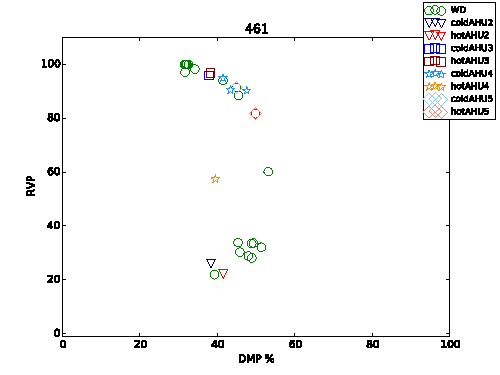
\includegraphics[width=0.45\textwidth,height=2.0in]{./figs/incorrectzone.pdf}
%                \caption{A Zone incorrectly classified by our methodology. Results projected in 2D}
%                \label{fig:incorrectzone}
%\end{figure}
%
%
%\begin{figure*}[ht!]
%\centering
%                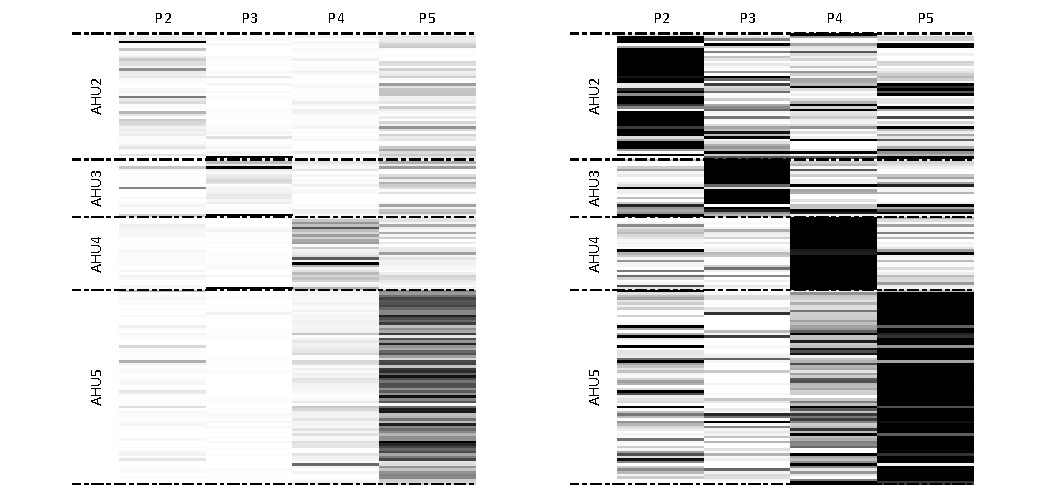
\includegraphics[width=0.90\textwidth,height=2.0in]{./figs/heatmap.pdf}
%                \caption{Heatmap}
%                \label{fig:heatmap}
%\end{figure*}

\begin{figure*}[ht!]
\centering
        \begin{subfigure}{0.30\textwidth}
                \centering
                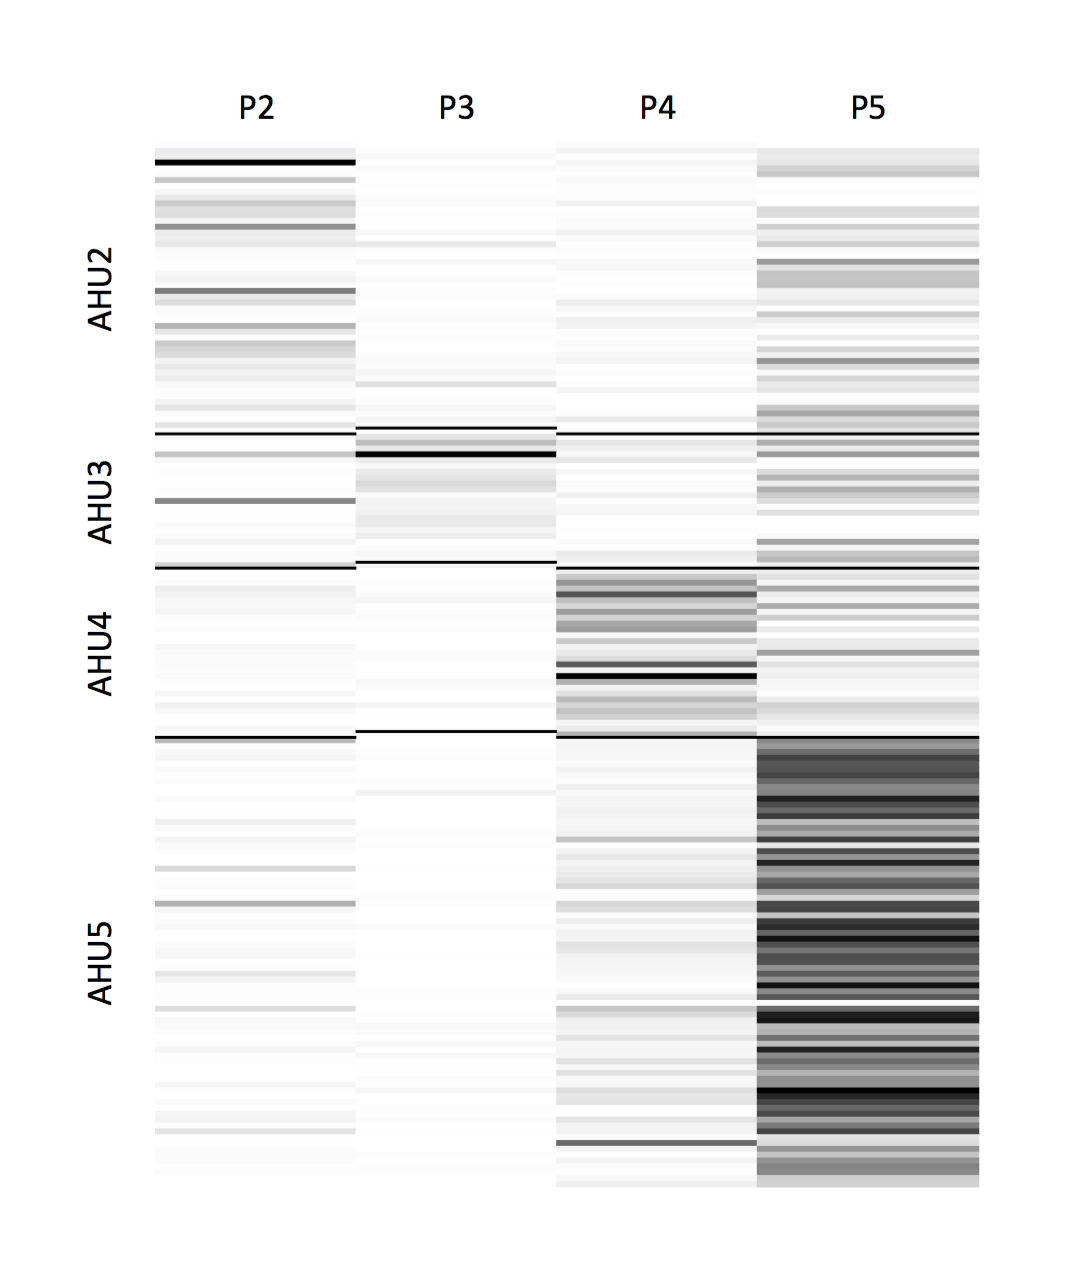
\includegraphics[width=\textwidth,height=2.0in]{./figs/columnnormalized.png}
                \caption{Treating each perturbation as a standalone experiment}
                \label{fig:columnnormalized}
        \end{subfigure}
        \hfill
        \begin{subfigure}{0.30\textwidth}
                \centering
                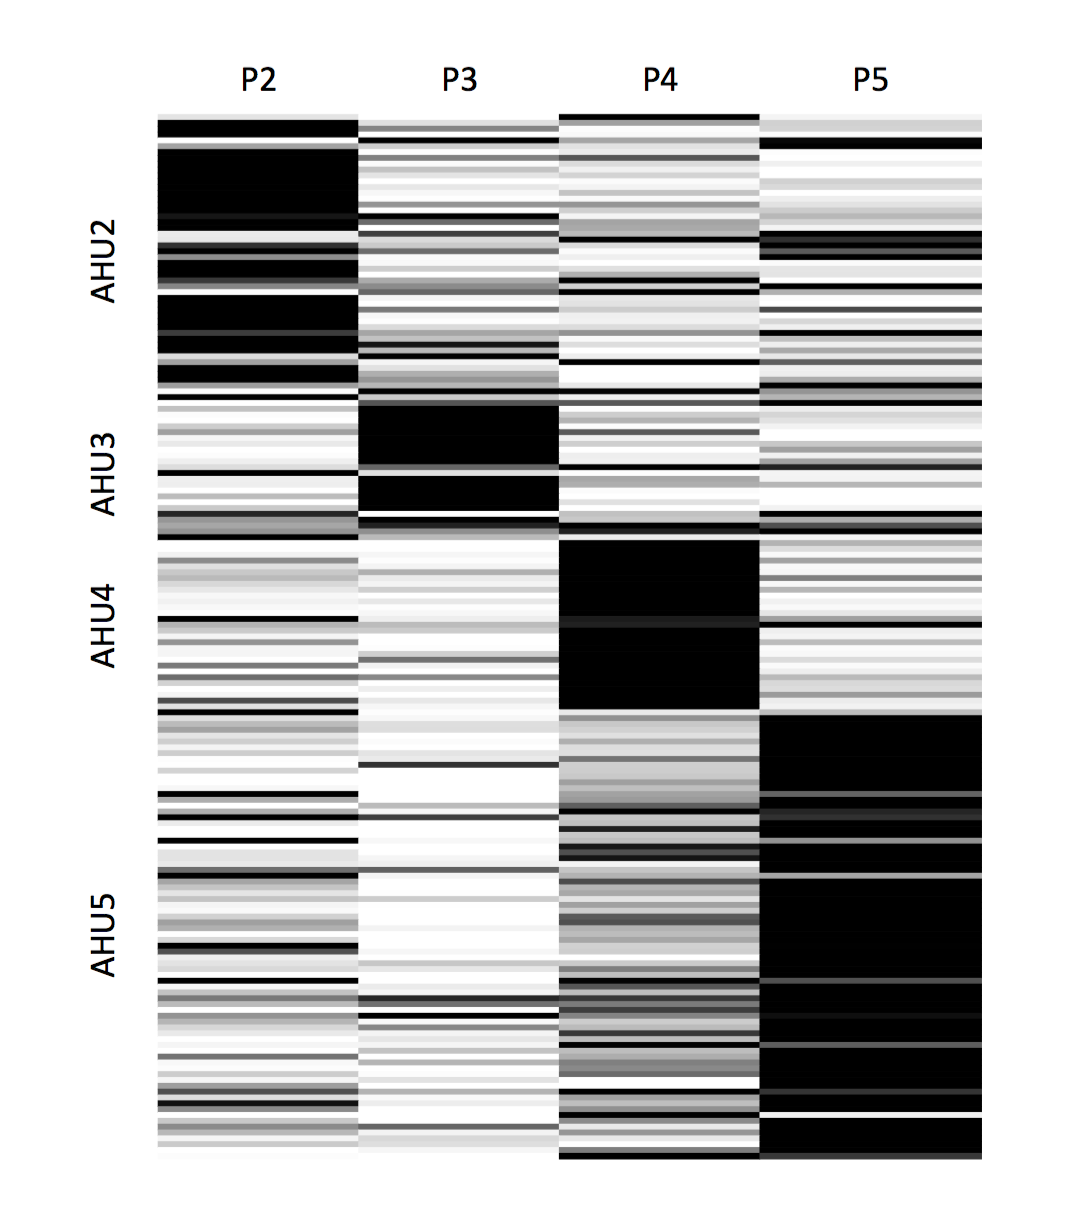
\includegraphics[width=\textwidth,height=2.0in]{./figs/rownormalized.png}
                \caption{Advantages of using a voting method}
                \label{fig:rownormalized}
        \end{subfigure}
        \hfill
                \begin{subfigure}{0.30\textwidth}
                \centering
                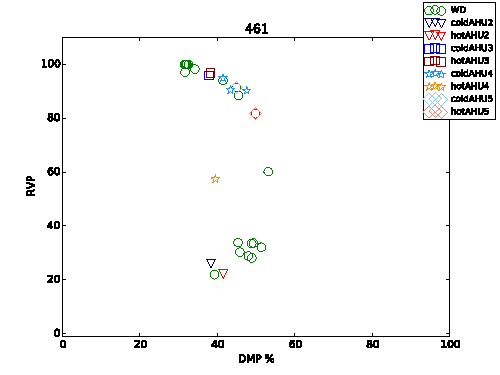
\includegraphics[width=\textwidth,height=2.0in]{./figs/incorrectzone.pdf}
                \caption{A zone incorrectly classified by our methodology. Results projected in 2D}
                \label{fig:incorrectzone}
        \end{subfigure}
\caption{Overview of perturbation statistics across all zones in a building}
\label{fig:active-learning}
\end{figure*}

The proposed methodology was applied to the building explored with the other methods. The results were encouraging, and the method correctly identified the relationship between VAV box and AHU in 79\% of the cases. There were three main groups of rooms that were incorrectly classified: 1) VAVs that showed no response to any perturbation, 2) VAVs that had a unexpected behavior, such as counter-intuitive responses to perturbations, 3) VAVs that responded more strongly to the perturbation of the ‘wrong’ AHU.
For instance Zone 308 (not shown here for brevity) presents a very tight distribution of variables, as DAM is at its minimum, and daily average RVP changes very little during all the periods. Further analysis of this case reveals very frequent oscillations (about 20 cycles per days) of RVP ranging between 0\% and 40\%. It is very likely that the control loop is out of tune for this room. This is likely the reason why the perturbation has no visible effect on the data. This is a misclassification of the first kind.

\begin{table}[ht]\scriptsize
 \caption{ Comparison of accuracy of the voting method and the independent scoring method}
 \label{tab:results}
\begin{tabular*}{0.40\textwidth}{|c|c|c|c|}
\hline
Accuracy/Precision & \multicolumn{2}{|c|}{Independent classification} & Voting \\ \hline
& Threshold=0 & Threshold=2 S.D & Max Value  \\ \hline
AHU 2 &	39\% / 31\% &	78\% / 68 \% &	85\% / 77\% \\
AHU 3 &	35\% / 16\% &	92\% / 85\% &	94\% / 77\% \\
AHU 4 &	22\% / 17\% &	92\% / 77\% &	92\% / 69 \% \\
AHU 5 &	48\% / 45\% &	80\% / 100\% &	86\% / 85\% \\ \hline
\end{tabular*}
\end{table}



On the other hand, zone 461 (Figure 2) shows a very wide distribution of points. The room seem subjected to large unmeasured disturbances. Some baseline weekdays reach max RVP (~100\%), while others use only a fraction of reheat (10-30\%). These unknown factors probably had a larger effect compared to the perturbation, causing the room to be misclassified (type 2).
The effects of adopting a voting system compared to scoring each perturbation individually can be seen in Table 3. The classification of each AHU individually, based on its corresponding perturbation, requires defining a threshold to compare the calculated metric to. Choosing the right threshold is challenging and hard to generalize. In Figure 3 each line represents a VAV box sorted by ground-truth AHU, while each column represents a perturbation of an AHU. The color in each cell is shaded proportionally to the value of the calculated metric, normalized by column. Darker values represent higher metric values and are used to associate the VAV box to the perturbed AHU. It is clear from the figure that each perturbation produces responses in multiple VAV boxes, some of which are not associated with the correct AHU. Choosing a threshold corresponds to choosing a min shade of grey that triggers the association with the AHU currently perturbed. Further, Figure 3 shows that perturbation 3 and perturbation 5 (in column) require a very different threshold to correctly classify the corresponding VAVs. In contrast, Figure 4 illustrates the clearer heat map generated with voting. Dark areas are more clearly defined and it is visually easier to identify which VAV boxes are associated to the AHUs.
In addition, if a room is classified in different ways under separate perturbations (e.g. belonging to two AHUs) then the classification conflict needs to be resolved. When a voting system is adopted, a room is classified in a univocal way. In Table 3 we show the accuracy of the independent classification with two thresholds and the voting method 


